\documentclass[10pt,twocolumn]{article}

% ------------------ PAQUETES ------------------
\usepackage[spanish]{babel}
\usepackage[utf8]{inputenc}
\usepackage[T1]{fontenc}
\usepackage{geometry}
\usepackage{graphicx}
\usepackage{amsmath, amssymb}
\usepackage{siunitx}
\usepackage{authblk}
\usepackage{abstract}
\usepackage{caption}
\usepackage{titlesec}
\usepackage{multicol}
\usepackage{hyperref}
\usepackage{currfile}
\usepackage{float}

\geometry{margin=1.8cm}

% ------------------ FORMATO DE SECCIONES ------------------
\titleformat{\section}{\large\bfseries}{\thesection}{1em}{}
\titleformat{\subsection}{\normalsize\bfseries}{\thesubsection}{1em}{}
\titleformat{\subsubsection}{\normalsize\bfseries}{\thesubsubsection}{1em}{}

% ------------------ TÍTULO ------------------
\title{\textbf{Aproximación inicial a las estrellas variables}\\Estudio del atlas de curvas lúminicas de estrellas variables elaborado por Igor Soszynski\\Entre otros}


% ------------------ AUTORES ------------------
\author[1]{Bruno Abello Laurent}

\affil[1]{Universidad de Los Andes, Departamento de Física, Colombia}

% Correos (puedes modificar)
\renewcommand\Authands{, }
\date{}

\begin{document}

\twocolumn[
\maketitle
\begin{center}
\small
\textit{Correo institucional:} \href{mailto:{b.abello@uniandes.edu.co}}{b.abello@uniandes.edu.co} \\
\end{center}

\begin{abstract}
\noindent

\end{abstract}

\noindent\textbf{Palabras clave:} 
\vspace{0.5cm}
]

% ------------------ CONTENIDO ------------------

\section{Introducción}

El presente documento es un informe detallado de las lecturas y trabajos del autor sobre su descubrimiento del mundo de las 
estrellas variables. Gracias al Atlas of Variable Star Light Curves, elaborado por Igor Soszynski y el trabajo sobre
estrellas binarias eclipsantes de Dan Brutoni, se puede realizar una introducción bastante completa al conocimiento que 
se tiene de estos fenómenos estelares. El único acercamiento práctico que se verá en este documento es la demostración 
del valor del ángulo con respecto al plano de observación que han de tener dos estrellas binarias para que podamos observar
su eclipsamiento.

El trabajo presentado a continuación se realiza para poder tener el conocimiento necesario para poder realizar aplicaciones.
Por ejemplo, se trabajará en la búsqueda de periodicidad y en la búsqueda de estrellas variables, a través de una serie de 
5 informes, con este siendo el primero. 

\subsection{Objetivos}

Los objetivos que tenemos, en términos simples, son los siguientes:
\begin{itemize}
    \item Aprender a entender la información específica que se puede obtener de una estrella variables
    \item Aprender a diferenciar los tipos de estrellas variables
    \item Entender qué condiciones se tienen que dar para observar estrellas eclipsantes desde un punto del espacio
\end{itemize}

Las secciones de problemas presentados y procedimiento se obvian en este informe puesto que no hay mayores problemas que se 
puedan presentar en la realización de este trabajo y no hay un procedimiento específico que se ha de seguir. Claro que vale 
la pena aclarar que se fue leyendo el atlas subsección a subsección, y se fueron anotando las observaciones directamente en 
este documento con el fin de estructurar todo a posteriori. 

\section{Resultados}

El lector se podrá preguntar por qué la definición de una estrella variable no se encuentra en la introducción de este documento.
Lo cierto es que el autor no sabía qué era una estrella variable antes de empezar a investigar, por lo que tiene más sentido poner
la definición de estrella variable como el primer resultado. 

Tanto en clase como en una búsqueda rápida por internet, se puede encontrar que una estrella variable es aquella estrella cuya magnitud
varía sistemáticamente con el tiempo. O sea, se le ve un cambio periódico y no aleatorio. No es difícil dar el salto de esto a que pueden 
haber distintas maneras en las que una estrella puede presentar ese fenómeno. Por ende, se denomina como extrínseca a aquella estrella
cuya magnitud varía debido a un agente externo, como una estrella binaria que a veces nos presenta toda su magnitud y a veces se eclipsa
para mostrar su magnitud como la de una sola estrella. Por el contrario, una estrella intrínseca es la que varía su magnitud sin influencia
externa. Puede, por ejemplo, estar titilando en tamaño, haciendo erupciones bruscas o estallando en una única y enorme explosión 
(\cite{clase_presencial, wikipedia_variable_star}). 

Evidentemente, la clasíficación se extiende más allá de esto. Revisaremos entonces los ejemplos estándar de estrellas variables.

\subsection{Sistemas Binarios eclipsantes}

Como dicho anteriormente, un tipo de estrella variable es aquella que es eclipsada por otro cuerpo celeste de manera periódica. 
Empezaremos por revisar algunos tipos de estas estrellas.

\subsubsection{Algol variables}

Este tipo de estrellas son posiblemente los más sencillos; ambas estrellas, o al menos la más luminosa, son esféricas.
Es sencillo imaginar que, debido a la distribución de estrellas eclipsantes en el universo, algunas van a tener sus 
eclipses mucho más visibles que otras. Las tipo Algol, justamente, muestran su eclipse de manera muy clara a través del tiempo;
su principio y su final. Al menos una a una. En la figura (Fig: ~\ref{NormalAlgol}) vemos un claro ejemplo de esto: un eclipse grande
en fases 0 y 1, donde la estrella más luminosa es ocultada por la menos luminosa, y otro más pequeño en fase 0.5, donde ocurre lo contrario. 
Esto es debido a que una estrella es más luminosa que otra, lo que ocurre en la  mayoría de los casos. El eclipse en fase 0.5 se puede 
ver desplazado si las órbitas de las estrellas son excéntricas (Fig: ~\ref{EccentricAlgol}).

\begin{figure}[H]
    \centering
    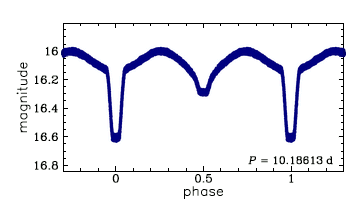
\includegraphics[width=0.8\linewidth]{../LightCurves/Algol/Normalita.png}
    \caption{Curva de magnitud con respecto a fase de un sistema binario eclipsante tipo Algol natural}
    \label{NormalAlgol}
\end{figure}

\begin{figure}[H]
    \centering
    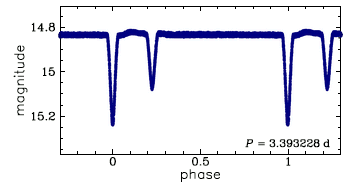
\includegraphics[width=0.8\linewidth]{../LightCurves/Algol/Excéntrica.png}
    \caption{Curva de magnitud con respecto a fase de un sistema binario eclipsante tipo Algol con órbitas eccéntricas}
    \label{EccentricAlgol}
\end{figure}

\begin{figure}[H]
    \centering
    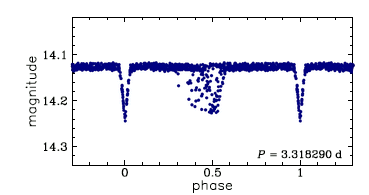
\includegraphics[width=0.8\linewidth]{../LightCurves/Algol/Aspidal.png}
    \caption{Curva de magnitud con respecto a fase de un sistema binario eclipsante tipo Algol con movimiento aspidal. }
    \label{AspidalAlgol}
\end{figure} 

Evidentemente, se complican más las curvas si la órbita, ya elíptica, de una de las estrellas, presenta movimiento aspidal, 
es decir que va rotando en su propio plano. Esto se traduce por una curva de luz borrosa en los eclipses y menos lineal
entre estos (Fig: ~\ref{AspidalAlgol}). Estas estrellas también presentan fenómenos más complejos, como el efecto de
reflección, los discos de acreción o la doble periodicidad. 

\begin{figure}[H]
    \centering
    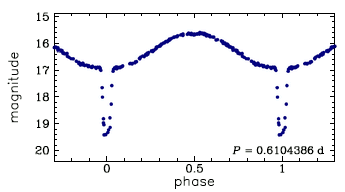
\includegraphics[width=0.8\linewidth]{../LightCurves/Algol/Reflexión.png}
    \caption{Curva de magnitud con respecto a fase de un sistema binario eclipsante tipo Algol con efecto de reflexión.
    Se observa un efecto tan intenso que el eclipse secundario es prácticamente invisible.}
    \label{ReflexiónAlgol}
\end{figure}

\begin{figure}[H]
    \centering
    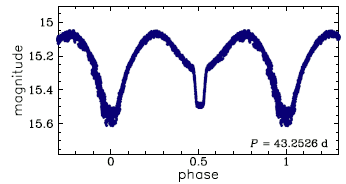
\includegraphics[width=0.8\linewidth]{../LightCurves/Algol/Accretion.png}
    \caption{Curva de magnitud con respecto a fase de un sistema binario eclipsante tipo Algol en el que una estrella
    posee un disco de acreción. Se observa como el eclipse primario es más largo que el secundario. }
    \label{AccretionAlgol}
\end{figure}

\begin{figure}[H]
    \centering
    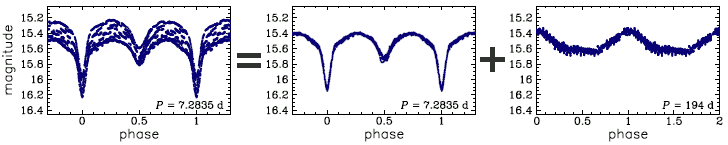
\includegraphics[width=0.8\linewidth]{../LightCurves/Algol/Double.png}
    \caption{Curva de magnitud con respecto a fase de un sistema binario eclipsante tipo Algol con doble periodicidad.
    Se ve cómo la gráfica principal, a la izquierda, es la suma de dos variaciones periódicas, que se pueden separar. }
    \label{DoubleAlgol}
\end{figure}

El primero ocurre cuando la diferencia en temperatura  de las estrellas es muy grande, y la luz de la estrella más 
caliente es absorbida y reflejada por la más pequeña. En consecuencia, el brillo aumenta por fuera de los eclipses
(Fig: ~\ref{ReflexiónAlgol}). Por otro lado, cuando una de las estrellas cuenta con un disco de acreción,
el eclipse que provoca es más largo que el eclipse provocado por su compañera, lo que se ve claramente en el 
gráfico (Fig: ~\ref{AccretionAlgol}). Por último, en 2003 (\cite{mennickent2003double}) se descubrió que podía
existir un sistema periódico, con otro periodo entre 20 y 50 veces más largo que el primero, de origen aún desconocido. 
En este caso, se pueden deconstruir los datos para obtener las gráficas de ambos fenómenos por separado(Fig: ~\ref{DoubleAlgol}).

\subsubsection{Beta Lirae variables}

El atlas describe a este tipo de estrellas como estrellas binarias cuya magnitud aparente cambia continuamente, y cuyos
miembros cuentan con diferencias significativas en su temperatura. Como recordaremos del inciso anterior, esto significa 
un cambio brusco entre el efecto del eclipse primario y el del eclipse secundario (Fig: ~\ref{NormalBLyrae}). Adicionalmente, estas estrellas tienen
forma elipsoidal debido a laa fuerza de oleaje de su compañera, con el atlas diciendo que puede ser que una de sus estrellas
llene su lóbulo de Roche \footnote{El lóbulo de Roche es la región del espacio alrededor de una estrella en un sistema 
binario en la que el material orbitante está ligado gravitacionalmente a dicha estrella. Si la estrella se expande más 
allá de su lóbulo de Roche entonces el material exterior al lóbulo es atraído por la otra estrella. \cite{wikipedia_lobulo_roche}}, 
haciendo que se dé una transferencia de masa a su compañera; una binaria semi-desligada.

Hay que notar que algunos de estos sistemas pueden verse afectados por el efecto O'Connell, probablemente asociado a la
transferencia de masa entre estrellas, en el cual un máximo de magnitud entre eclipses es menor que el otro (Fig: ~\ref{OconBLyrae}). 

\begin{figure}[H]
    \centering
    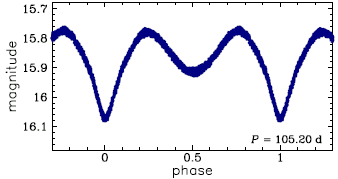
\includegraphics[width=0.8\linewidth]{../LightCurves/BetaLyrae/Normal.png}
    \caption{Curva de magnitud con respecto a fase de un sistema binario eclipsante tipo Beta Lyrae. Se nota, a 
    comparación de un sistema Algol, que los eclipses y máximos se presentan como un continuo más que como dos 
    funciones disyuntas.}
    \label{NormalBLyrae}
\end{figure}

\begin{figure}[H]
    \centering
    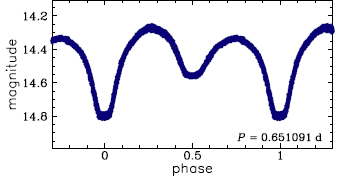
\includegraphics[width=0.8\linewidth]{../LightCurves/BetaLyrae/Ocon.png}
    \caption{Curva de magnitud con respecto a fase de un sistema binario eclipsante tipo Beta Lyrea con efecto 
    O'Connell. Se aprecia que el primer máximo en fase positiva es mayor al segundo, dando lugar a un efecto O'Connell
    positivo. El negativo invierte el orden, y es mucho más raro.}
    \label{OconBLyrae}
\end{figure}

\subsubsection{W Ursae Majoris}

La particularidad de estas estrellas es que ya llenaron su lóbulo de Roche: están intercambiando materia y por ende están
a la misma temperatura, relativamente. Esto hace que los eclipses sean supremamente similares entre sí, y que no se pueda
diferenciar claramente entre el final de uno y el inicio del otro(Fig:~ \ref{NormalWUrsaeM}). FALTA HABLAR DE SCORPII

\begin{figure}[H]
    \centering
    
\includegraphics[width=0.8\linewidth]{../LightCurves/WUrsaeMajoris/Normal.png}
    \caption{Curva de magnitud con respecto a fase de un sistema binario eclipsante tipo W Ursae Majoris. Se ven 
    los eclipses de impacto muy similar en la parte inferior del gráfico, así como los máximos de inicio y final de eclipse
    en la parte superior.}
    \label{NormalWUrsaeM}
\end{figure}

\subsection{Estrellas variables pulsantes}

Ahora pasamos a otro tipo de estrellas variables, aquellas que son solitarias y pulsan por otros artificios de la física. 

\subsubsection{Ceféidas clásicas}

Estas estrellas, Ceféidas de tipo 1, son jóvenes, masivas, y pulsan radialmente. La humanidad las conoce muy bien, y 
debido a esto actúan como una especie de faro en el universo; permiten medir distancias muy bien gracias a sus
bien conocidas relaciones entre periodo y magnitud absoluta. Estas estrellas pulsan en modo fundamental, o en el 
primer o segundo armónico. En el modo fundamental, el periodo de una estrella está entre 1 y 200 días, aunque
generalmente sean de uos pocos días. En la mayoría, existe una correlación entre la curva de luz y los periodos
de oscilación: la progresión de Herztprung (\ref{Progresion}). Esta se manifiesta como un chichón en la rama 
descendiente de las curvas de luminosidad de las ceféidas de periodos cortos. A medida que el periodo se alarga, 
la anomalía progresa hacia el máximo de la curva, o sea hacia atrás en fase. No existe cuando el periodo es superior 
a los 20 días (Fig: ~\ref{NormalCefeid}). Nótese que el Atlas cataloga algunas estrellas con amplitudes muy pequeñas, 
donde esta progresión es poco visible. 

\begin{figure}[H]
    \centering
    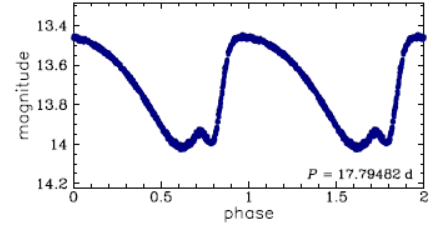
\includegraphics[width=0.8\linewidth]{../LightCurves/Cefeidas1/fundamental.png}
    \caption{Curva de magnitud con respecto a fase de una cefeida clásica en modo fundamental de oscilación.
    La progresión de Hertzprung es visible justo antes de un máximo. Suponemos que, puesto que el periodo 
    aproxima los 20 días, ya nos encontramos del otro lado de la evolución de este fenómeno.}
    \label{NormalCefeid}
\end{figure}

\begin{figure}[H]
    \centering
    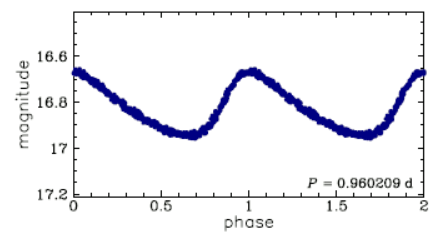
\includegraphics[width=0.8\linewidth]{../LightCurves/Cefeidas1/PrimerModo.png}
    \caption{Curva de magnitud con respecto a fase de una cefeida clásica oscilando en el primer armónico. Vemos que
    no hay progresión de Herztprung y que la amplitud de la oscilación es menor que para una estrella en el modo fundamental.}
    \label{PrimerCefeid}
\end{figure}

\begin{figure}[H]
    \centering
    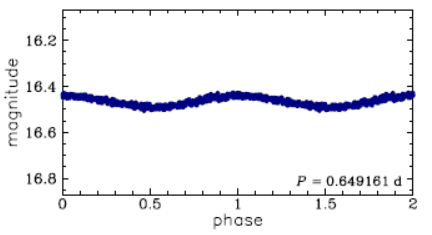
\includegraphics[width=0.8\linewidth]{../LightCurves/Cefeidas1/SegundoModo.png}
    \caption{Curva de magnitud con respecto a fase de una cefeida clásica oscilando en el segundo armónico. La amplitud de 
    la oscilación es muy pequeña, y la oscilación en sí es prácticamente sinusoidal.}
    \label{SecondCefeid}
\end{figure}

En el primer armónico, las amplitudes suelen ser más pequeñas y las curvas más simétricas(como en los previamente estudiados
sistemas binarios.). Su periodo depende de la metalicidad del medio, pero el atlas no da una escala para esto de manera
directa. Sin embargo, sí menciona periodos que no pasan de los 10 días y que no tienen límite inferior, teniendo una conexión 
suave y directa con estrellas tipo Delta Scuti, estrellas que no nos interesan el día de hoy, pero que podemos suponer de periodos
muy bajos. La frontera entre estos tipos de estrellas fue puesta por el OGLE en 0.24 días (Fig: ~\ref{PrimerCefeid}). Lógicamente, 
al ver cómo ha evolucionado la amplitud en estas estrellas, el segundo armónico tiene una amplitud muy pequeña. La mayoría existe 
en lugares con pocos metales, y son tan raras que el OGLE ha detectado menos de 100 entre las nubes de magallanes menor y mayor 
(Fig: ~\ref{SecondCefeid}).

El lector podrá haberse dado cuenta de que es posible que las estrellas pulsen en varios modos. En estos casos, lo único curioso 
que pasa es que las curvas  de luz se ven más gruesas, especialmente al mezclar el modo fundamental y el primer armónico. La mayoría
del tiempo, se obtienen estrellas con primer y segundo armónico, que presentan curvas enos dramáticas que la anterior combinación. 
Cuando se combinan estos tres modos de oscilación, aunque sea muy raro(10 ejemplares catalogados), las oscilaciones se vuelven caóticas
y las curvas parecen tener pelos: no presentan una continuidad suave como en anteriores ejemplos. 

Por último, es importante notar que hay ejemplos de ceféidas en un sistema binario. Estos fenómenos le permitieron a los físicos 
resolver el problema que tenían entre lo que mostraban los modelos de pulsación y los modelos de evolución estelar para la masa
de una estrella. Gracias al sistema binario, se puede conocer directamente la masa de la cefeida y solucionar estas discrepancias 
de manera tajante. 



\subsection{Progresion de Herztprung} \label{Progresion}

\section{Conclusiones}

\section*{Comentarios al margen}

\bibliographystyle{apalike}
\bibliography{refs}
\end{document}